\chapter{Additional Video Prediction Results}
\label{app:video_prediction_additional_results}

This appendix provides additional results for the video prediction evaluation in Section~\ref{sec:video_processing_results}. The main chapter reports the human-labeled accuracy evaluation using \acrshort{iou} and sensitive-region coverage. The results below are included as supporting material.

\section{Temporal Coverage Test}
Before evaluating prediction accuracy against human-labeled ground truth, a temporal coverage test was performed. The purpose of this test was not to measure exact tracking accuracy, but to measure whether Kalman-based prediction preserved active \gls{bounding box}es across frames where full detection was not executed.

Since full detection is only executed on selected frames, a detection-only manifest would only contain detected boxes on those frames. Automatic Kalman-based prediction was therefore compared with this detection-frame-only estimate to evaluate whether it preserved the \gls{bounding box}es across non-detection frames.

\begin{table}[H]
\centering
\begin{tabular}{rccc}
\toprule
\textbf{\texttt{detect\_every}} & \textbf{Detection calls} & \textbf{Detection-only} & \textbf{Manifest with prediction} \\
\midrule
1  & 261.00 & 99.44\% & 99.44\% \\
2  & 130.67 & 50.02\% & 99.63\% \\
5  & 52.33  & 20.09\% & 99.63\% \\
10 & 26.33  & 10.15\% & 99.17\% \\
\bottomrule
\end{tabular}
\caption{Average frame coverage across the three tested videos. ``Detection-only'' estimates the percentage of frames that would contain boxes if boxes were only used on frames where full detection was executed. ``Manifest with prediction'' shows the percentage of frames with active boxes after Kalman-based prediction has propagated boxes between detection frames.}
\label{tab:video_temporal_coverage_appendix}
\end{table}

This substantially increased bounding-box coverage when detection was run less frequently. With \texttt{detect\_every = 10}, the detection-frame estimate was 10.15\%, while the prediction-based manifest maintained 99.17\% coverage on average. This confirms that the prediction step filled the gaps between detection frames and produced continuous boxes for later review and redaction.

However, this metric should be interpreted only as a temporal coverage result. It shows whether boxes were present in the frame-wise manifest, but it does not show whether the boxes were accurately aligned with the sensitive objects. For this reason, the main video evaluation in Section~\ref{sec:video_processing_results} uses human-labeled ground truth, \acrshort{iou}, and sensitive-region coverage as the primary accuracy results.

\section{Worst-Frame Example}

Figure~\ref{fig:video_prediction_worst_frame_appendix} shows the lowest-quality frame found in the \texttt{car\_video} sequence when using \texttt{detect\_every = 10}. This example was selected from the human-labeled evaluation and illustrates a difficult case with several nearby moving vehicles.

\begin{figure}[H]
\centering
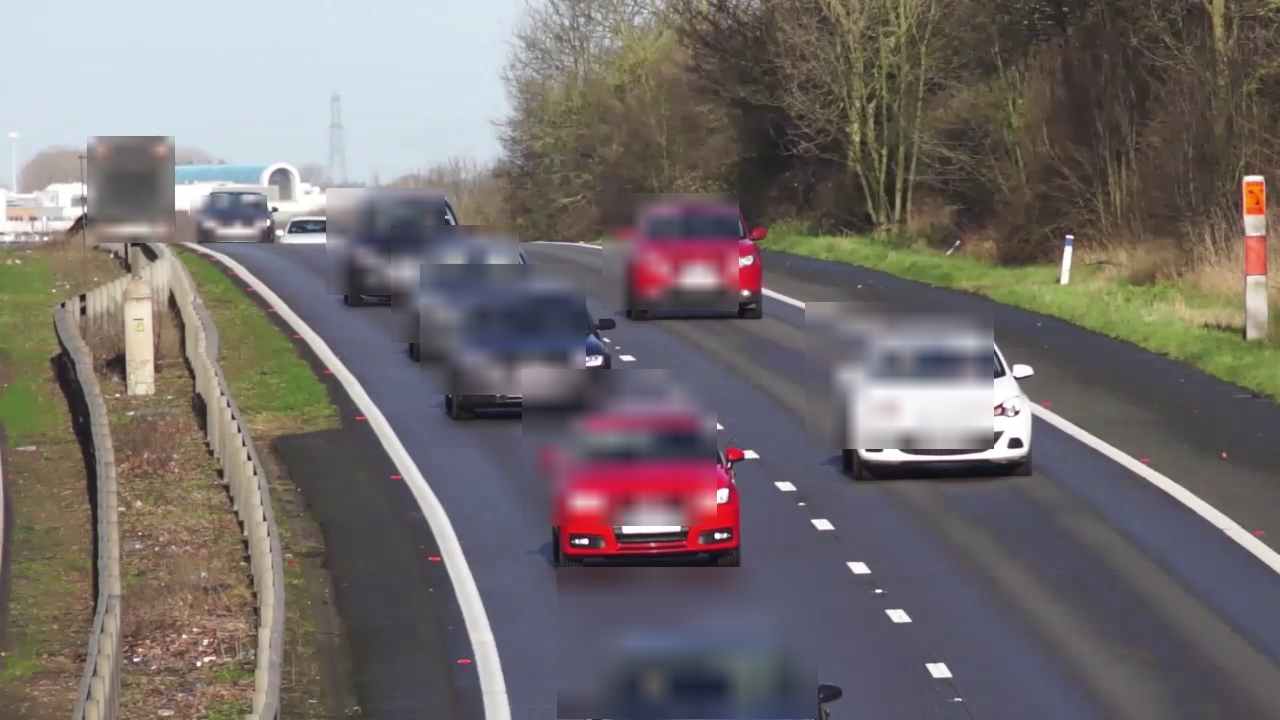
\includegraphics[width=0.85\textwidth]{figures/images/chapter-11/car_kalman_worst_frame.png}
\caption{Worst-frame example from the \texttt{car\_video} sequence using \texttt{detect\_every = 10}. The frame contained nine human-labeled vehicle boxes and ten predicted boxes. The mean \acrshort{iou} was 0.5245, while mean sensitive-region coverage was 0.7469. This illustrates that long prediction intervals can reduce localization accuracy in frames with several nearby moving objects.}
\label{fig:video_prediction_worst_frame_appendix}
\end{figure}

This example shows why both \acrshort{iou} and sensitive-region coverage were used in the main evaluation. The predicted boxes still cover large parts of the sensitive regions, but the alignment is less precise than in easier frames. This makes the frame useful as a qualitative example of the limitations of longer prediction intervals.